\documentclass[titlepage]{article}
\usepackage[utf8]{inputenc}

% used for enhanced justification
\usepackage{microtype}

\usepackage[margin=0.6in]{geometry}

% used for indexing
\usepackage{index}
\makeindex

% used for images
\usepackage{graphics}
\graphicspath{ {./images/} }

% used for adjusting alignment for images
\usepackage[export]{adjustbox}

% used to stop images floating in strange ways
\usepackage[section]{placeins}

% used for nicer headers
\usepackage{fancyhdr}

% math packages
\usepackage{amssymb}
\usepackage{mathtools}
\usepackage{natbib}
\usepackage{amsmath}
\usepackage{amsfonts}
\usepackage{amssymb}

\title{Eternity}
\author{Tyler Shanks, Danny Roux, Andrei Serban, Vatsa Kartik Shah,\newpage William Robinson, Nicholas Simo, Arash Singh}
\date{June 14 2021}

\begin{document}
\begin{titlepage}
   \begin{center}
       \vspace*{1cm}

       \Huge
       \textbf{Eternity}

        \vspace{0.5cm}
        \Large
        Nicholas Simo, Danny Roux, Arash Singh,
        \\Vatsa Kartik Shah, William Robinson, Tyler Shanks, Andrei Serban
       
       \vspace{6cm}
        Introduction to Software Engineering
        \\COMP 354
        \\Pankaj Kamthan

        
       \vspace{1.5cm}
        
        \Large

       \vfill
            
       \vspace{0.8cm}
     
       
\includegraphics[width=0.4\textwidth]{images/concologo.png}

       Gina Cody School of Computer Science and Software Engineering\\
       Concordia University\\
       Canada\\
       June 14 2021
            
   \end{center}
\end{titlepage}



\fancyfoot{\thepage}

\tableofcontents
\addtocontents{toc}{\protect\enlargethispage{\baselineskip}}
\newpage

\section{Introduction}
    \subsection{Glossary}
        \begin{itemize}
            \item Arccos(x): The arccosine of x is when the cosine function of x is reversed when x is in between or equal to -1 and 1. When the cosine is set up to y is equal to x, the arccosine of x equals the reversed cosine function of x, which is equal to y. \cite{arccos}
            \begin{center}
                $arccos(x) = cos^{-1}(x) = y$
            \end{center}
            \item Euler’s Number: Denoted by e, Euler’s number is a constant in mathematics approximating to 2.71828. It should be noted that e is an irrational number.\cite{boundless}
            \item Irrational Number: A number is said to be irrational if it cannot be written as a ratio of two integers. An example of this is Euler’s number. \cite{wolfram}
            \item Integer: A number that is whole. \cite{merriam}
            \item Exponent: Given a number x and exponent y, the result given by the expression $x^y$ is the value of x multiplying itself y times (i.e. the result of $2^3$ gives $2 * 2 * 2 = 8$). It should be noted that the x and y variable can themselves be functions. However, the same principle still applies. The same principle applies to a constant to a power of x (i.e $2^{0.98x+3}$).
            \item Hyperbolic Sine: Hyperbolic function which traces a hyperbola. Calculated through formula: (where e is Euler’s Number) \cite{encyclopaedia}
            \begin{center}
                $sinh(x) =  \frac{e^x - e^{-x}} {2}$ 
            \end{center}
            \item Logarithmic function: It is the inverse of an exponential function. When using the log function without an explicitly defined base, the assumed base will be 10. For simplicity sake, the natural log known as $log10(x) = ln(x)$ will not be used within the documentation.\cite{dawkins}
            \begin{center}
                $f(x) = log_b(x) = b^{f(x)}x$ 
            \end{center}
            \item  Mean Absolute Deviation: It is the average distance between each data point and the mean for a specific dataset. \cite{khan}
            \item Standard Deviation: A measure of how spread out the data is compared to the average. Denoted with $\sigma$. \cite{students}
        \end{itemize}
        
    \subsection{Functions}
        \begin{enumerate}
            \item $\begin{aligned}[t]
                arccos(x)
            \end{aligned}$
                Worked on by Will
            \item $\begin{aligned}[t]
                ab^x
            \end{aligned}$
                Worked on by Andrei
            \item $\begin{aligned}[t]
                log_{b}(x)
            \end{aligned}$
                Worked on by Shanks
            \item $\begin{aligned}[t]
                MAD
            \end{aligned}$
                (Mean Absolute Deviation) Worked on by Vatsa
            \item $\begin{aligned}[t]
                \sigma
            \end{aligned}$
                Worked on by Nicholas
            \item $\begin{aligned}[t]
                sinh(x)
            \end{aligned}$
                Worked on by Arash
            \item $\begin{aligned}[t]
                x^y
            \end{aligned}$
                Worked on by Danny
        \end{enumerate}

    \subsection{Collaboration Patterns}
        \paragraph{}
        Over the course of the beginning weeks of COMP 354, our team has met for weekly meetings every Friday at 9:00pm. Throughout these meetings, our team has had pertinent discussions regarding each team member’s role in the group, what every team member needed to accomplish for the following week and develop questions to ask the teacher assistants. These questions are then asked to the teacher’s assistant during lab times.
        
        \paragraph{}
        We use a group chatting platform called Discord to communicate and host meetings. We have also decided to use Github to host our software code. Github allows each team member to share the code they are working on. In the future, this will allow our team to check up on each other’s work and offer advice to one another if needed. Lab times are also used for further discussion if needed with our team. Every member of our team has been present to every single lab time.

\section{Materials \& Methods}
    \subsection{Interviews}
        \subsubsection{Questions}
            \begin{enumerate}
                \item Name? Age? Profession? Level of education?
                \item What mathematics are involved in your day to day life?
                \item What type of calculator is suitable for you?
                \item What functions do you expect a calculator to have?
                \item Would you enjoy having a customizable calculator? Such as different coloured buttons or UI.
                \item Do you prefer having options such as "dark mode", "light mode" or having the option to choose?
                \item Should there be documentation to explain how each function works within the calculator as well as how to interact with the UI?
                \item How accurate do you expect the calculator to be? For example, to the 6th decimal place.
                \item Would you like to be able to keep a history of calculations and their results?
                \item For functions that require you to have several different values for each variable, would you rather they be entered one by one or all at once (in an array)?
                \item Do you want to be able to use the calculator with a command line interface?
                \item Would you like to swap between the pages for the scientific functions and the normal elementary arithmetic functions?
                \item As for the display of the calculator, is it important for you to have a display that can display fractions and symbols as you would write them on paper?
                \item How much would you be willing to pay for this calculator?
                \item Are there any other features that you'd like this calculator to have?
            \end{enumerate}

        \subsubsection{Responses}
            \begin{itemize}
                \item Julies Benson - Car Salesman
                    \begin{enumerate}
                        \item My name is Jules Benson and I am 43 years old. I am a car salesman for Audi. My level of education is a bachelors degree in marketing.
                        \item Normally, I do math when I’m near my desk sitting down with a customer. Math in my job involves calculating the total cost of the vehicle, adding or subtracting vehicle options cost, and more importantly, calculating the monthly payment of the vehicles and the interests.
                        \item The most difficult calculation that I have to do during the whole day is calculating interests that involve a lot of percentages. So for my needs, a basic calculator, without any scientific function is sufficient.
                        \item I expect that a calculator has the ability to do basic calculations obviously. A percentage button would be helpful, that way I wouldn’t have to multiply everything by 100 each time I’m taking a percentage.
                        \item Not necessarily, It wouldn’t change much in my job, I’m looking for practicality over aesthetics.
                        \item My job is during the day, and the dealership is very bright as well, so I don’t really need a dark mode, but I wouldn’t mind it for those winter evenings when the sun goes down early.
                        \item Some documentation would be helpful just to know if there’s some things I previously didn’t know that a calculator can do.
                        \item I expect the calculator to be accurate to the 2nd decimal, which is needed when calculating interests on monthly payments.
                        \item Yes, that would be a good functionality. Sometimes customers are hesitating between different cars and different payment plans, so it will be practical to go back and see the previous calculation for comparison.
                        \item I don’t think I’ll be using that function but if anything, I would want them to be entered one by one.
                        \item I don’t know anything about programming, I am not very tech savvy. So, I don’t want to use it with a command line interface.
                        \item I will most likely be using arithmetic functions, but in some rare case that I end up using scientific functions, it would be a good idea to add a swap between pages just to separate the two functionalities.
                        \item Yes, that would be very helpful, since I wouldn’t have to use my brain too much on plugging in the calculator.
                        \item Around \$20
                        \item I mentioned that a percentage button would be helpful for me, so that’s one thing I would like the calculator to have
                    \end{enumerate}
                \item Chad Smith - Grade 10 Student
                    \begin{enumerate}
                        \item I'm 16 years old, and I'm in grade 10. I don't really have a profession.
                        \item As a high school student, the mathematics which I mostly use is algebra and geometry. But some students including me take advanced math classes which allows me to work on more complex functions like the gamma function.
                        \item I’d like a scientific calculator.
                        \item The calculator should at least have basic arithmetic functions like addition, subtraction, multiplication and division. And along with that it should have some transcendental functions like the logarithmic function, gamma function and arccos(x).
                        \item Yes, having a customizable calculator would allow me to stand out from other students at my school and would make my calculator very unique.
                        \item I would prefer light mode during day-time and dark-mode during nights. So, the option of having both would be the best.
                        \item Yes, a proper user guide explaining all the functions would be helpful.
                        \item I need accuracy to the 4th decimal at least.
                        \item Yes, a recent history of the calculations and their results would be really helpful. Since I’m a student, I work on several problems simultaneously, so going back and checking my previous answers would be really helpful.
                        \item Entering all values at once would be less time consuming and I’d prefer that.
                        \item No, the command line interface for a calculator doesn’t seem necessary to me.
                        \item Swapping between the pages again and again seems very tiring. I’d like it if all the functions are available on the same page.
                        \item I honestly don’t mind either. I’m comfortable with fractions as well as decimals.
                        \item I’m an unemployed 16 year old high school student. So for the calculator we discussed, I could pay max. \$15-\$20
                        \item It’ll be great if the calculator is mobile as well as computer friendly.
                    \end{enumerate}
                \item Shaunna Ross - Sales Representative
                    \begin{enumerate}
                        \item Hello, my name is Shaunna Ross, I am 46 years old. I have a high school degree which has led me to be a sales representative at a retail store.
                        \item At the retail store my daily math consists of simple addition for sales, subtraction for a customer’s return and using percentages to calculate the weekly deals that certain articles of clothing in the store could have. The numbers that come from the computer are crucial to the success of the store, as if those numbers are incorrect, the store can be penalized heavily.
                        \item I just need a simple calculator, not very complicated. I do not need any of the very high math functions that look complicated. Concise is key.
                        \item Well, I definitely think that calculators should always have the basic ones, like adding, subtracting. Even functions I would necessarily use, like multiplication and division are still important to have.I also require the calculator to provide me with 2 decimal places because some clients may pay in cash, and I quickly need to know how much change I may need to give them back. Also as I mentioned before, I need percentages to supply my customers with proper savings and deals.
                        \item It would be interesting to have this functionality. I would love to have this, as I could customize the calculator to fit the theme of my store, and maybe have some customers give their thoughts on an artistic calculator. I could add labels, store icons and colors similar as inside my store.
                        \item I would prefer light mode, as I feel it would be more expressive to how I want my store to run. Although having a dark mode could also be a great addition.
                        \item I personally would like some documentation, as I am not great with computers, and so having documentation could help me a great deal. Also, If I am ever in a hurry, knowing how the buttons work can help me resolve issues that arise.
                        \item I need the calculator to always provide me with 2 decimal places. It is crucial that I provide my customers with exact change if they pay in cash.
                        \item Having a history is extremely important that the calculator has this as a function as I want to be able to provide evidence for customers that what they paid is what they gave me. It is also important to know how much money I have received during the day as I sell more products.Also, it will help me determine If a customer is lying to me for certain transactions. SO yes I would like to keep a history of the calculations.
                        \item I will not really need a functionality for this ever I believe, but if I ever do, I would like to have them one by one.
                        \item To be honest, I do not know what a command line interface is. I am not good with computers, so I would love a simple place where I can press buttons and the actions happen. That tells me that the calculator is working, and that is all I need.
                        \item I do not need a page for scientific functions, even though they could be interesting to use. The basic functions on the front page is perfect for my needs.
                        \item The display should have my number with 2 decimal places. That is perfect for me, since that is what I will use on a daily basis. Fractions are not needed, as I also need to have the customers know how much they are paying. Symbols I would like to have, as they can show me the steps in the purchases or returns of the customers.
                        \item I only need some very easy functions, therefore I am not willing to pay an arm and a leg for a calculator.
                        \item A cool feature that I can request is to have the calculator showcase a simple phrase or couple of words when the calculator is not in use. Adding a “Welcome!” to the calculator will make me buy this product just that much more. The phrase will please customers and illustrate to them that I put a lot of thought into my work environment. This will in turn allow them to trust that they are receiving great clothes.
                    \end{enumerate}
                \item Pierre Cyr - General Contractor
                    \begin{enumerate}
                        \item My name is Pierre Cyr, I am 60 years old. I work as a general contractor for a construction company, and I studied at the Chambre des Notaires du Québec.
                        \item As a general contractor, I use mathematics when working on budgets for construction contracts, which involves finding the quantities required of each material, calculating the total prices for those materials, and how much it will cost for the workers. When on a construction site, I use mathematics to calculate the different distances and areas.
                        \item Something that is simple to use and intuitive. I don’t want to fiddle with a calculator to get the results, I just want it to work. Also not something too small either.
                        \item I expect the “normal” calculator functionalities, plus, minus, multiplication, and division, along with the exponents functions and the trigonometric functions, as I use those quite frequently either when making construction plans or when on the job site, to make sure that the angles are correct.
                        \item I don’t really see the point of customizing the colors of the calculator, as long as the functions are labeled correctly.
                        \item Dark mode is easier on the eyes to use, so I prefer dark mode, but I don’t mind if it is normal.
                        \item As long as the functions are labeled correctly, I don’t think that the documentation on what the button does is necessary, unless the functionality is not intuitive.
                        \item I expect a calculator to have at least 4 decimal positions to get the most accurate result possible, but the more the better. If there aren’t enough then I could get rounding errors, and that would be really bad.
                        \item Keeping a history would help greatly, to check if one of the calculations was incorrect and check on past results.
                        \item I think that in an array would be better, since if I make a mistake entering the results, I can go back to change it, whereas one by one I would have to wait to finish to enter all results before fixing it.
                        \item I would not really have a use for that functionality, no.
                        \item I don’t really have a utility in that, unless the scientific functions really take up a lot of space.
                        \item It would really help if the equations would show up like that, yes. It would be more visually clear if there’s a mistake in the calculation. But how easy would it be to navigate? Because I can move up and down now, it might be a bit difficult to navigate.
                        \item I wouldn’t expect to pay anything just for a calculator, except if it was able to calculate things more easily than using a normal calculator, but even then I wouldn’t spend more than \$5 for it.
                        \item Something that’s always annoyed me with normal calculators is that if there’s a mistake in the calculation, like I forgot to put something after a plus, it waits until I press equal to tell me there was a mistake. Why not let me know beforehand? Also, if you keep track of the history of the calculations, it would be nice to be able to assign a title to the calculation, so that I can remember what it was for. Conversion of units would be quite useful as well, for example to go from sq2 to m2.
                    \end{enumerate}
                \item Jim Turner - Welder
                    \begin{enumerate}
                        \item My name is Jim Turner, age 39, and I graduated high school and then did a DEP in welding.
                        \item As a welder, we use a lot of basic math and some trigonometry in order to cut and weld the right size pieces. The calculator has to be precise, otherwise the final product that we are welding won’t hold the proper shape, and the safety and stability of the structure could be compromised.
                        \item Normally a basic calculator is sufficient enough but we do prefer a scientific calculator since it has the trigonometry functions pre installed.
                        \item As a welder, built in trigonometry functions such as sine, cosine, and tangent would be adequate.
                        \item I would like to have some buttons customized such as a larger equal sign. Buttons should be large so that we have no problems pushing the wrong numbers or functions. I would also like to have a delete button in addition to a clear button so if I make a mistake on one number, I don’t have to clear and start all over. This would help me save time during my work.
                        \item I prefer the option to have both because the lighting in my workplace varies.
                        \item Yes, some basic documentation could be useful.
                        \item As a welder, to the 4th decimal would be ideal. Though less or more would be okay as well.
                        \item Yes, definitely. The history would be very important and it would also be helpful if I can copy/paste the history.
                        \item As a welder, one by one would be best to be able to input each exact custom number and do the steps.
                        \item No, this is not necessary for welders as it will be too time consuming and the average welder does not have that high of computer literacy to use that interface. It’s best to keep it simple.
                       \item Yes, this would be helpful because sometimes we just need basic elementary functions and other times we need the scientific ones. Being able to switch back and forth will make it faster and easier to use when we just need the basic functions.
                        \item No, it’s not because a fraction can mean different values in relation to measurements. It’s easier to just have the numbers and decimals.
                        \item I would be willing to pay up to \$40 if it had all the functions I needed and didn’t drain my device's battery as this is a tool I will be using daily.
                        \item If the calculator is a software/app, it would be a cool feature if we could send a calculation to another user (colleague) so they could see the exact formula and answer. It would also be neat if it had a built-in unit conversion function.
                    \end{enumerate}
                \item Evelyn S. Jones - Security Researcher
                    \begin{enumerate}
                        \item Hello my name is Evelyn S. Jones, I’m 25 years old. I currently work as a Security researcher while I am completing my Masters degree in Information System Security.
                        \item I work with all kinds of math on a daily basis. From basic addition, subtraction, to complex polynomial operations involving both exponential and logarithmic functions. I also use the hexadecimal and binary system often in my work, these are particularly important for me.
                        \item Since my work requires me to switch back and forth between number systems, I would require a fancier calculator than most. A scientific calculator would be able accomplish most of my needs though, having hex and binary conversion would save me a lot of time therefore having a programmer function to allow for that to happen would be great.
                        \item I would expect basic arithmetic functions that allows for at least 9 digits to be shown. At its most basic level it should cover Real Numbers and not deal with imaginary ones. As calculators become more powerful I would expect many more functions that would include polynomials and other statistical functions, like what scientific calculators provide.
                        \item Having a customizable calculator would be pretty cool however I really don’t care too much for having that option. To me a calculator is a tool so having a “pretty” tool just to compute equations isn’t something that really matters to me.
                        \item Personally I prefer dark mode but having the option of both light mode and dark mode is much better. Sometimes I do prefer to switch to light mode because of where my desk is, the light shines on it pretty brightly and I get quite a bit of glare.
                        \item If the calculator has unorthodox functions then yes it should definitely have documentation to explain how they work or how they are laid out. If the calculator has a UI I think it should have documentation since on occasion you get strange layouts that are unintuitive.
                        \item In terms of accuracy I would prefer it to be until the 9th decimal place.
                        \item Having the ability to keep the history of calculations and their results would be great. I often get side tracked and then lose my train of thought so having the history is a great way for me to keep pace on my work in case of sudden distractions.
                        \item As long as I’m made aware of the order of the variables, I would love to have the ability to enter each value in an array format. That way I can double check my values to ensure that they are in fact correct.
                        \item I would prefer for this calculator to have a command line interface. I find that it’s much easier to manually type out the entire equation than to have a pretty GUI.
                        \item I am not a fan of having separate pages for the scientific and basic functions since I use them all in conjunction. If there are many functions then I can understand the need for pages or an “alternative/shift” button that would allow for the use of other functions to compute.
                        \item It is not important for that functionality to be present. However, I can see that if regular people use the calculator they might be more inclined to respond yes to that question. Personally it doesn’t matter to me since programming has made me care less for such functionalities.
                        \item I would not spend anymore than \$50.
                        \item The single feature I would love to have is a decimal to binary/decimal to hex converter that also works vice versa. I go back and forth between these number systems so having them available to me would save me a great amount of time.
                    \end{enumerate}
                \item Ricciardo Rossi - Junior Formula 1 Race Engineer
                    \begin{enumerate}
                        \item Hello, my name is Ricciardo Rossi. I am 38 years old, and I am a junior race engineer for Scuderia Toro Rosso Formula 1 team. I graduated with a master’s degree in software engineering from Sapienza University of Rome. My masters focused mainly on algorithm design with special focus on analysis and optimization.
                        \item I think most people do not realize this, but a race engineer needs to be a jack of all trades that works in liaison with almost all departments including the drivers. Communication needs to be clear and concise to convey important information from the technical department to the driver for them to push the car to the limit. Mathematics is at the center of it all. I do not need to know all the specifics, but I need to have a general idea of what people of various departments are talking about. Therefore, the mathematics involved may be arithmetic, trigonometry, calculus, probability, optimization, and many others. It depends on the day.
                        \item Most of the complicated calculations are already done through the various proprietary software that we use. However, I also have two physical calculators on my desk, just to make sure if one breaks I have a backup. If need be, I use my phone’s calculator for some quick arithmetic if I am on the go.
                        \item A calculator should have general functions such as: basic arithmetic, algebra, logarithms, and trigonometry. In certain situations, the software calculators on my laptop can be an inconvenience to use at certain moments such as when travelling. If the handheld calculator has more key functions such as standard deviation, probability, and calculus, it would be even better.
                        \item I don’t really need any customizable feature in terms of colors for the buttons and UI. However, it would be nice if the customizability extends to complicated functions that general calculators do not have. I guess in that scenario, I would just use a scientific calculator instead haha.
                        \item When I am not having meetings with various departments, I am in front of a screen:  laptops, factory hardware, phones, calculators, and various others. To protect my eyes, I always use them while in dark mode.
                        \item Yes, documentation increases efficiency.
                        \item Honestly, the more accurate the calculator, the better it is for me. Every part of a formula 1 car needs to be designed and made perfectly. Any minute error in our calculations can cost us the race or cause the car to fail. I would therefore expect more than 12 decimal places.
                        \item Yes, that would be a great addition. Keeping history will enable be to backtrack to double check my calculations.
                        \item I see the advantage for both scenarios. I would use the array feature when I have a lot of information to input and vice versa, one by one, when I only have 2 or 3 variables to enter.
                        \item As a race engineer, it would be a great addition to have any calculator. However, most of our complicated calculations are done by our own software, so I would use the command line feature sporadically.
                        \item I believe that would be a great feature to have in order to maintain the logs of your previous calculations.
                        \item It is not important for me.
                        \item I have some flexibility in terms of price. If the calculator gets the job done with no impressive features I am willing to spend \$50. However, if the calculator is able to impress me with its capabilities, I am willing to go up to \$100.
                        \item I would like to be able to export all my calculations and data to files so that I am able to share them with my colleagues. 
                    \end{enumerate}
            \end{itemize}
            
        \subsection{Personas}
            %\begin{minipage}{\linewidth}
                \begin{figure}[!htb]
                    \centering
                    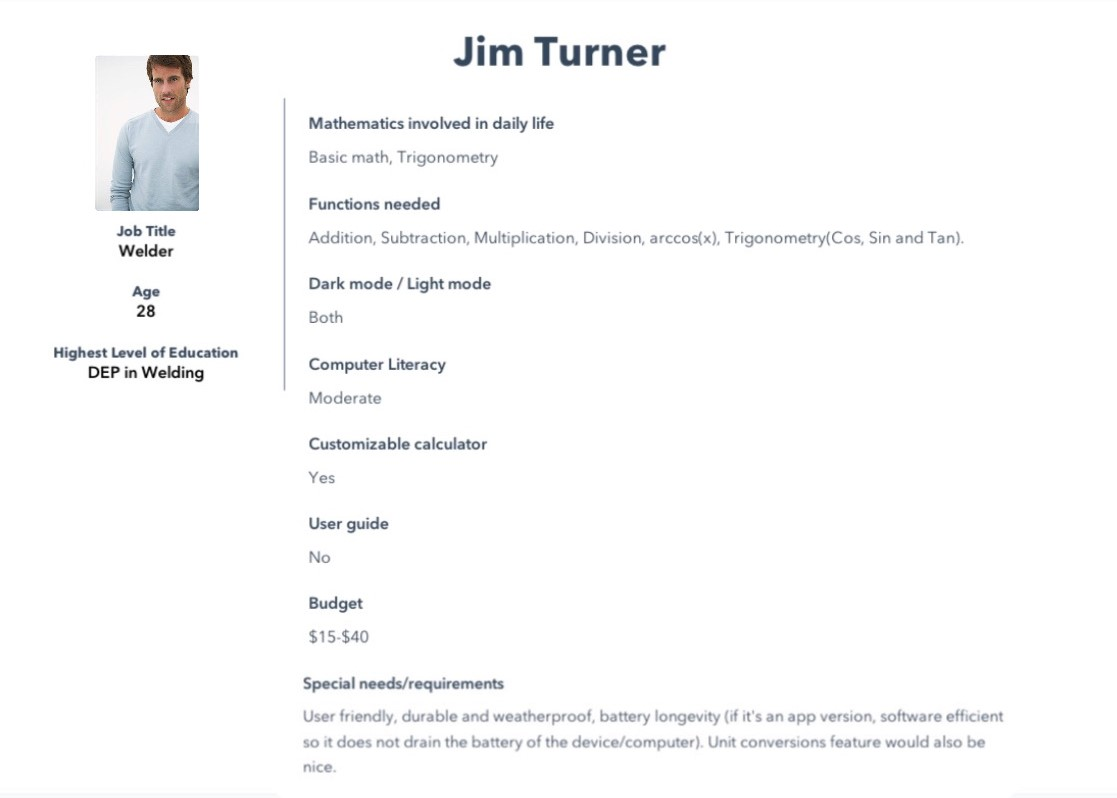
\includegraphics{images/Jim-Turner.JPG}
                \end{figure}
            %\end{minipage}
            \begin{figure}[!htb]
                \centering
                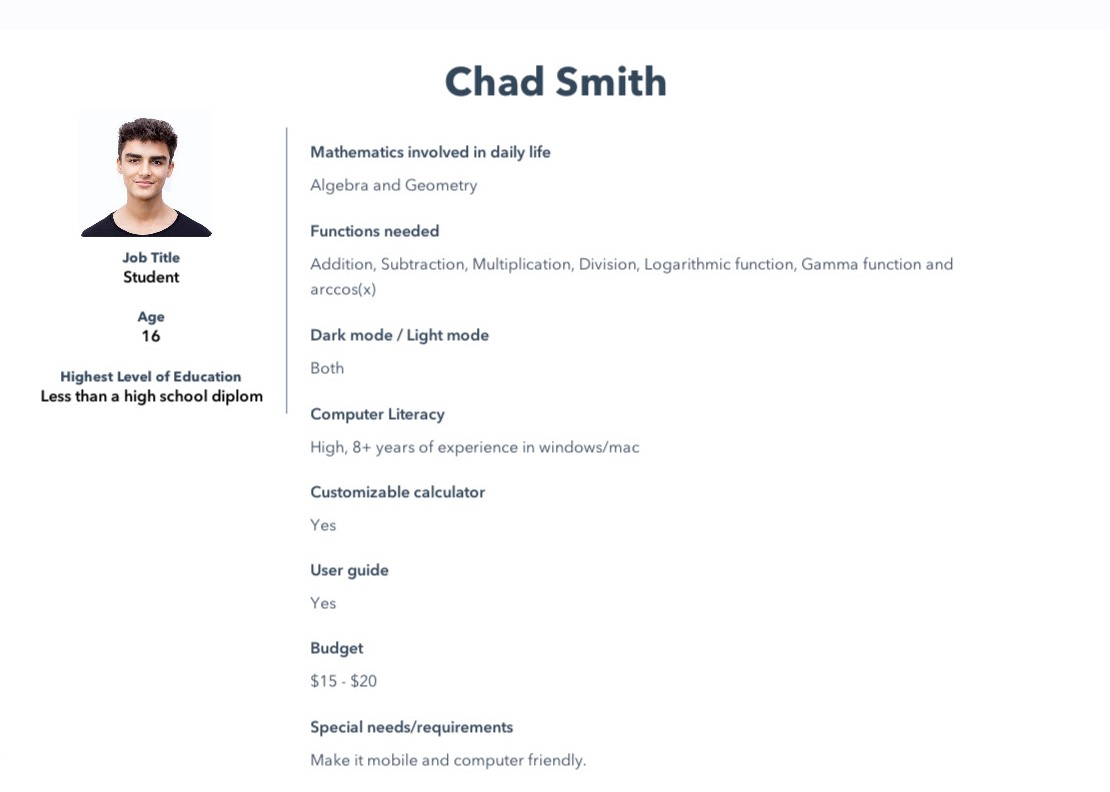
\includegraphics{images/Chad-Smith.JPG}
            \end{figure}
            \begin{figure}[!htb]
                \centering
                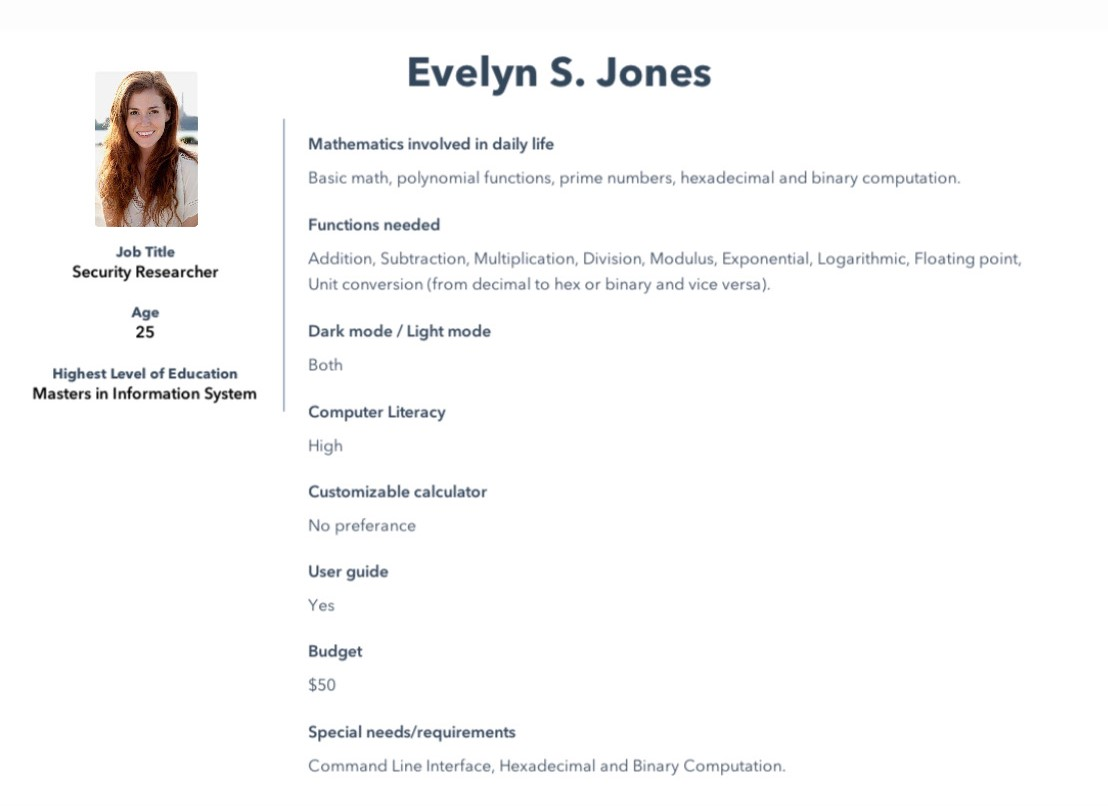
\includegraphics{images/Evelyn-S-Jones.JPG}
            \end{figure}
            \begin{figure}[!htb]
                \centering
                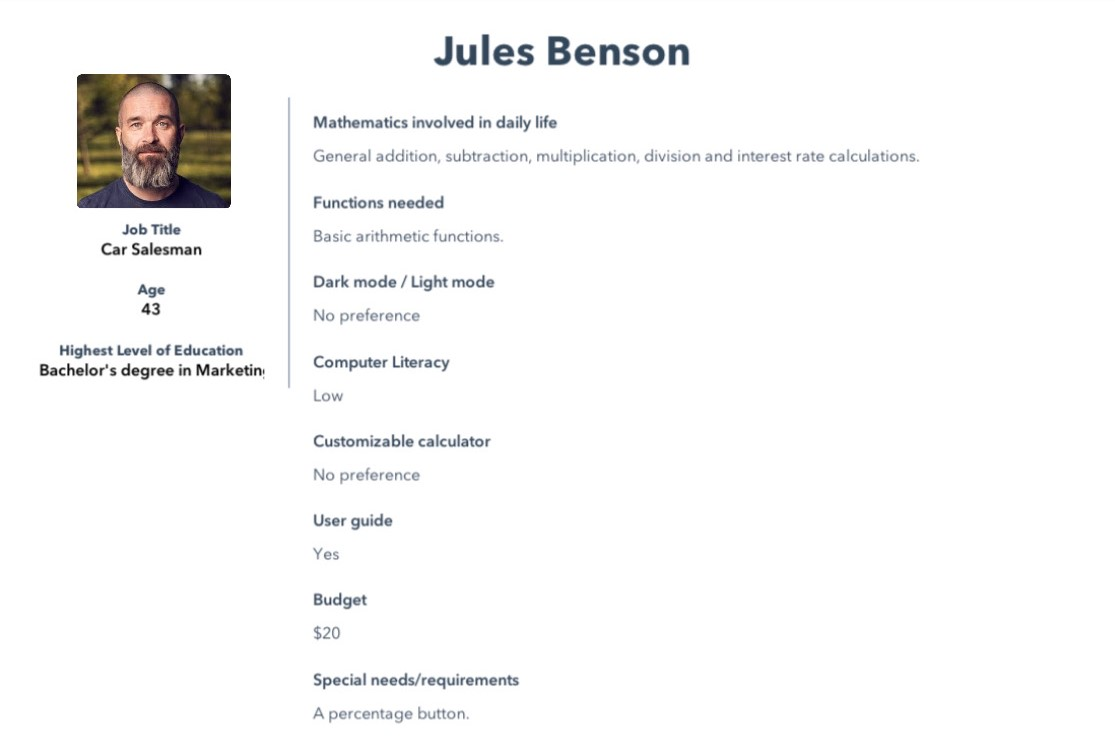
\includegraphics{images/Jules-Benson.JPG}
            \end{figure}
            \begin{figure}[!htb]
                \centering
                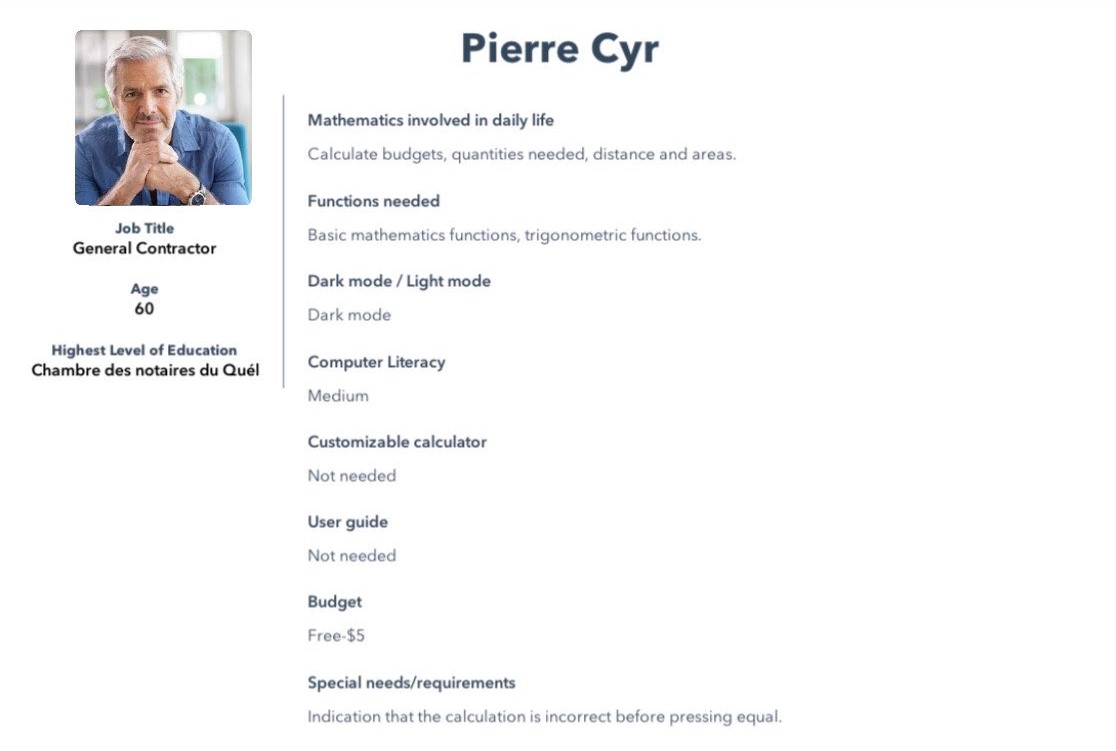
\includegraphics[scale=0.5]{images/Pierre-Cyr.JPG}
            \end{figure}
            \begin{figure}[!htb]
                \centering
                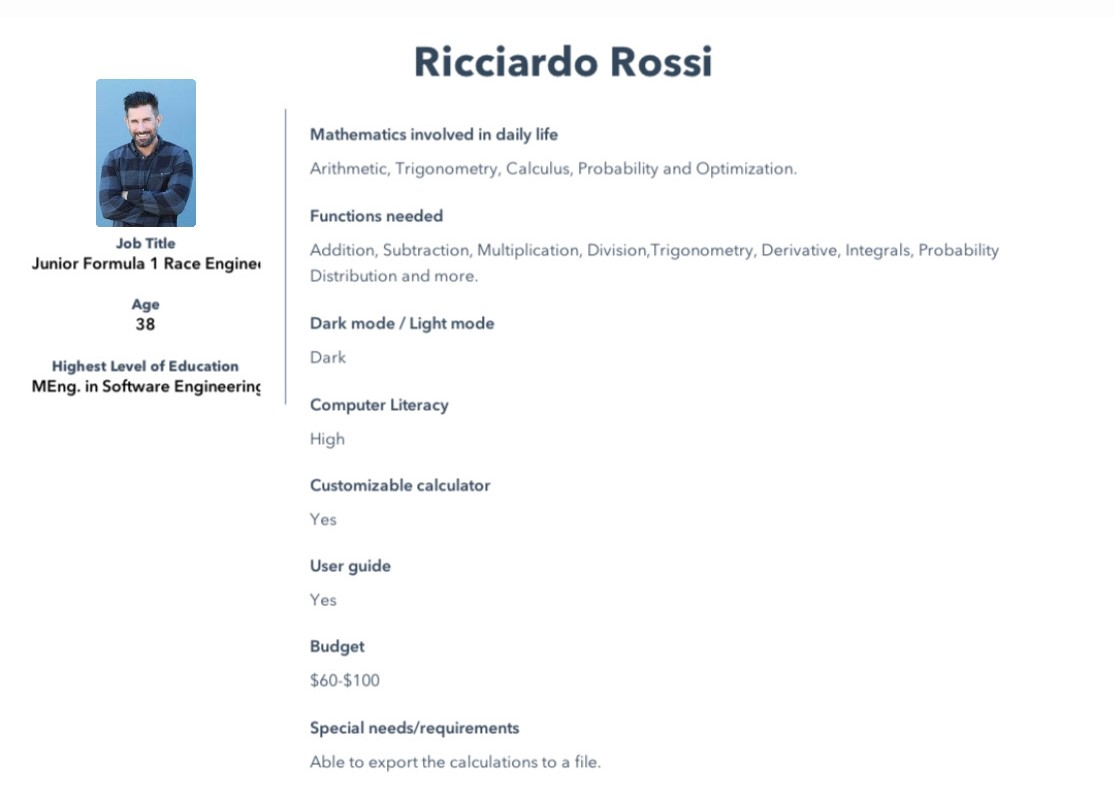
\includegraphics{images/Ricciardo-Rossi.JPG}
            \end{figure}
            \begin{figure}[!htb]
                \centering
                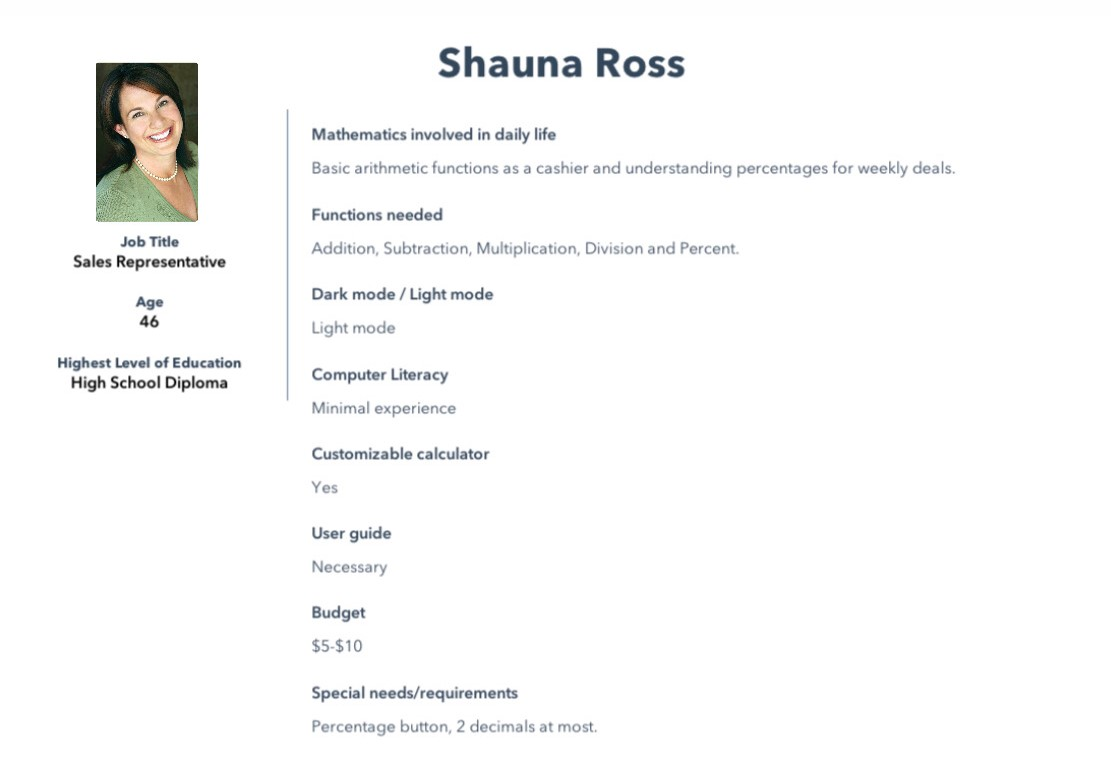
\includegraphics{images/Shauna-Ross.JPG}
            \end{figure}
            \FloatBarrier
        
        \subsection{Use Cases} 
            \begin{figure}[!htb]
                \centering
                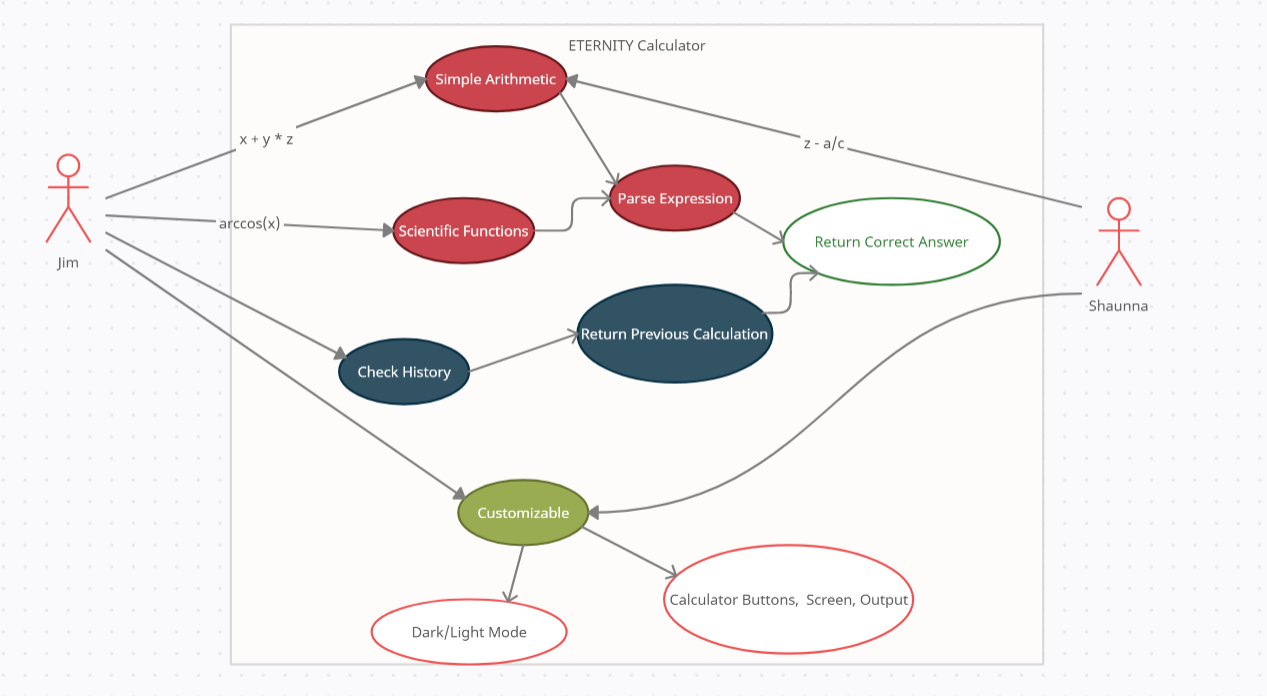
\includegraphics[scale=0.65]{images/UseCases.PNG}
            \end{figure}
            \FloatBarrier
            
\section{Analysis}
        \paragraph{}
        The aim of this project is to create a scientific calculator with transcendental functions built from scratch. 7 potential users of this calculator were interviewed. And the interviews were based on 15 pre-determined questions.

       \paragraph{}
        It is clearly evident from the interviews that most of our interviewees prefer to have basic math functions like addition, subtraction, multiplication and division and, some transcendental complex functions like $arccos(x)$, $ab^x$, $log_b(x)$, $\gamma ()$, $MAD$ (Mean Absolute Deviation), $\sigma$, $sinh(x)$ and $x^y$ in the calculator. Hence, a scientific calculator with the above-mentioned functions would be the most appropriate calculator and would cater everyone’s needs. 
        
        \paragraph{}
        Next, we notice that some people prefer to have Dark mode, and some prefer to have Light mode in their calculator. We’ll give an option to switch between both on Eternity. The given data also suggests that most of our interviewees have little to no computer literacy, so Eternity would come with a very easy and user-friendly interface and would also come with a User Guide. The User Guide would have documentation to explain how the functions work and how the basic structure of the calculator is laid out. Another important aspect of the calculator is its accuracy.
        
        \paragraph{}
        The interviews indicate that Jules and Shaunna expect the calculator to have accuracy to the 2nd decimal, whereas, Chad, Pierre, and Jim expect to have accuracy to the 4th decimal at least. Therefore, Eternity would have accuracy to the 4th decimal. Also, it is evident from the interviews that the potential users of the calculator would like to keep a history of the calculations and their results. We plan to add this feature in the calculator too. Some functions like MAD  requires users to input multiple values for each variable, so we asked the interviewees if they would like to enter these numbers all at once or one by one and we got mixed responses. Jules, Shauna and Jim would prefer one by one, Chad, Pierre and Evelyn would like to enter all the values at once, and Ricciardio would like the option to choose from both.
        
        \paragraph{}
        In addition, it is obvious from the interviews that the interviewees do not feel the need of the command line interface and therefore Eternity won’t have one. However, the potential users of this calculator would like to swap between the pages for the scientific functions and the normal arithmetic functions. Next question in the interview was about the budget and how much these interviewees were willing to pay for a calculator like Eternity. Evelyn and Ricciardio had a comparatively higher budget of \$50 and \$60-\$100 respectively. Whereas the other interviewees were ready to pay somewhere in between \$0 to \$40. The final question in the interview was if these interviewees had any other features they’d like to add in the calculator, and we received varied responses. Jules would like a percentage button in the calculator, Chad would appreciate it if the calculator was mobile and computer friendly and Shaunna would like a “Welcome” message on the calculator as that would please the customers at her shop into believing that she puts a lot of thought into her work environment. Pierre thinks that indication that the calculation is incorrect before pressing equal is important as it saves a lot of time. She and Jim also think that unit converters would be a great addition to Eternity. In addition to that, Jim would also like the calculator to have a longer battery life and be user friendly, durable and weatherproof. Evelyn thinks that a decimal to binary/decimal to hex converter would be a great feature to add in the calculator. And finally, Ricciardo would like to export all his calculations and data to files so he can share it with his colleagues.
            
        \paragraph{}
        In conclusion, the interviewees would like the Eternity to have all the basic functions along with some transcendental functions. They would also like to have a user guide along with the calculator and are willing to pay up to \$100 for the application.

\newpage
\section{References}
\bibliography{References}
\bibliographystyle{IEEEtran}


\end{document}
